\section{Auswertung}
\label{sec:Auswertung}

\subsection{Bestimmung  der Tiefe und der Größe von Fehlstellen}

Die Höhe des Acrylblockes beträgt $8,01\,$cm und die Schallgeschwindigkeit in Acryl ist $c_A=2730 \, \symup{\frac{m}{s}}$.
Die gemessene Zeit eines A-Scans ohne Fehlstelle beträgt $t =59,12\, \symup{\mu}$s.

Mit Gleichung (5) wird die Höhe $h$ des Acrylblockes bestimmt.
\begin{align*}
  h = \frac{1}{2} c_A t = 0.0807 \symup{m} = 8.07  \symup{cm}
\end{align*}

Die so berechnete Höhe ist größer als die abgemessene Höhe, da der Ultraschall nicht ausschließlich durch den Acryblock läuft, sonder auch durch die
Schutzschicht der Sonde. Aus den beiden Höhen wird die Differenz $\Delta s$ berechnet:
\begin{align*}
  \Delta s = h - 8,01 \symup{cm} = \SI{6e-4}{\meter}
\end{align*}


Die mit der Schieblehre abgemessenen Abstände der Fehlstellen zu der oberen $(s_o)$ und unteren $s_u)$ Kante werden in Tabelle 1 dargestellt. Die Nummerierung der
Fehlstellen entspricht dabei der gleichen wie in Abbildung 1. Zusätzlich werden auch die mit dem A-Scan bestimmten Laufzeiten $(t_o \text{und} t_u)$ für die
die beiden Strecken, sowie die daraus resultierenden Strecken $(s_o' \text{und} s_u')$, in dieser Tabelle dargestellt.
\begin{table}[H]
  \centering
  \caption{Gemessene Abstände der Fehlstellen in dem Acrylblock.}
  \label{tab:spannung1}
  \begin{tabular}{c c c c c c c}
    \toprule
  Fehlstelle & $s_o/$cm & $s_u/$cm & $t_o/\symup{\mu}$s & $t_u/\symup{\mu}$s & $s_o'/$cm & $s_u'/$cm  \\
    \midrule
    1  &  1,905 & 5,97 & 14,44 & 43,97 & 1,91 & 5,94    \\
    2  &  1,74 & 6,15 & 13,23 & 45,20 & 1,75 & 6,11    \\
    3  &  6,11 & 1,33 & 45,18 & 9,84  & 6,11 & 1,28    \\
    4  &  5,40 & 2,18 & 40,42 & 16,50 & 5,46 & 2,19    \\
    5  &  4,63 & 3,01 & 34,37 & 22,55 & 4,63 & 3,02    \\
    6  &  3,89 & 3,89 & 28,86 & 28,90 & 3,88 & 3,89    \\
    7  &  3,08 & 4,66 & 22,91 & 34,85 & 3,07 & 4,70    \\
    8  &  2,29 & 5,48 & 17,08 & 40,58 & 2,27 & 5,48    \\
    9  &  1,49 & 6,18 & 11,27 & 46,43 & 1,48 & 6,28    \\
    10 &  0,70 & 7,17 & 5,43  & -     & 0,68 & -     \\
    11 &  5,55 & 1,58 & 40,99 & 11,57 & 5,54 & 1,52    \\
    \bottomrule
  \end{tabular}
\end{table}

Dabei wurde für die Strecken $s_o' \text{und} s_u'$ die zusätzliche Strecke $\Delta s$ bereits abgezogen. Für die zehnte Fehlstelle konnte
kein Wert für $t_u$ gemessen werden, da die elfte Fehlstelle diese überdeckt.

Die Größe $d'$ der Fehlstelle wird durch $d' = h - s_o' - s_u'$ bestimmt. In Tabelle 2 wird die Größe $d'$ der Fehlstellen und die
Größe $d$ der Fehstellenangegeben. Dabei gilt $d = h - s_o - s_u$. Außerdem wird die relative Abweichung $\Delta d$ dargestellt.

\begin{table}[H]
  \centering
  \caption{Dicke der Fehlstellen.}
  \label{tab:spannung1}
  \begin{tabular}{c c c c}
    \toprule
  Fehlstelle & $d/$cm & $d'/$cm & $\Delta d/ \%$  \\
    \midrule
    1  &  0,14 & 0,16 & 14,3    \\
    2  &  0,12 & 0,15 & 25,0  \\
    3  &  0,57 & 0,62 & 8,8   \\
    4  &  0,43 & 0,36 & -16,3  \\
    5  &  0,37 & 0,36 & -27   \\
    6  &  0,23 & 0,24 & -4,3   \\
    7  &  0,27 & 0,24 & -11,1   \\
    8  &  0,24 & 0,26 & 8,3   \\
    9  &  0,34 & 0,25 & -26,5   \\
    10 &  0,14 & -    & -    \\
    11 &  0,88 & 0,95 & 8,0   \\
    \bottomrule
  \end{tabular}
\end{table}


\subsection{Bestimmung des Auflösevermögen}
Die Messergebnisse und die daraus errechneten Abstände der Messung der ersten beiden
Fehlstellen mit der 4 MHz Ultraschallsonde werden analog zu obigen Ausführungen in Tabelle \ref{tab:4} aufgeführt.

\begin{table}[H]
  \centering
  \caption{Gemessene Abstände der ersten beiden Fehlstellen in dem Acrylblock mit der 4 MHz Ultraschallsonde.}
  \label{tab:4}
  \begin{tabular}{c c c c c c c}
    \toprule
  Fehlstelle & $s_o/$cm & $s_u/$cm & $t_o/\symup{\mu}$s & $t_u/\symup{\mu}$s & $s_o'/$cm & $s_u'/$cm  \\
    \midrule
    1  &  1,95 & 5,97 & 14,21 & 43,67 & 1,88 & 5,90    \\
    2  &  1,74 & 6,15 & 13,08 & 44,86 & 1,73 & 6,06    \\
    \bottomrule
  \end{tabular}
\end{table}

Dabei wurde wieder für die Strecken $s_o' \text{und} s_u'$ die zusätzliche Strecke $\Delta s$ bereits abgezogen.

In Tabelle \ref{fig:3} werden wieder die daraus errechneten Größen sowie die abgemessenen Größen der Fehlstellen,
sowie die bestehende Abweichung dargestellt.

\begin{table}[H]
  \centering
  \caption{Dicke der Fehlstellen bei Messung mit 4 MHz Ultraschallsonde.}
  \label{tab:3}
  \begin{tabular}{c c c c}
    \toprule
  Fehlstelle & $d/$cm & $d'/$cm & $\Delta d/ \%$  \\
    \midrule
    1  &  0,09 & 0,23 & 155,6    \\
    2  &  0,12 & 0,22 & 83,3  \\
    \bottomrule
  \end{tabular}
\end{table}

Die Abweichungen sind also wesentlich größer als bei der 2 MHz Sonde. 

\subsection{Bestimmung der Abmessungend er Störstellen mit dem B-Scan}

Für den B-Scan ergeben sich folgende Bilder.

\begin{figure}[H]
  \centering
  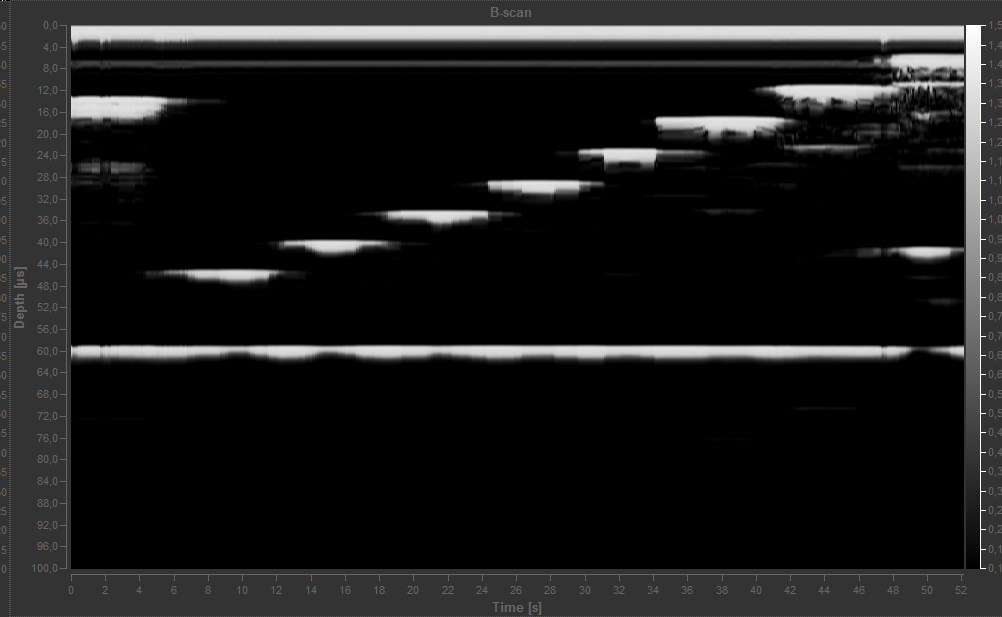
\includegraphics[height=5cm]{BScanoben.PNG}
  \caption{Abbildung des B-Scans von der oberen Kante.}
  \label{fig:acryl}
\end{figure}

\begin{figure}[H]
  \centering
  \includegraphics[height=5cm]{B-Scanunten.PNG}
  \caption{Abbildung des B-Scans von der unteren Kante.}
  \label{fig:acryl}
\end{figure}

Die mit dem B-Scan betimmten Laufzeiten und die daraus resultierenden Strecken werden in Tabelle 3 dargestellt.
Die Größe der Fehlstellen wird erneut aus den Strecken berechnet und ebenfalls in Tabelle \ref{tab:2}, mit zugehöriger Abweichung
zu den abgemessenen Werten, dargestellt.

\begin{table}[H]
  \centering
  \caption{Berechnete Werte bei einem B-Scan.}
  \label{tab:2}
  \begin{tabular}{c c c c c c c}
    \toprule
  Fehlstelle & $t_{B,o}/\symup{\mu}$s & $t_{B,u}/ \symup{\mu}$s  & $s_{B,o}/$cm & $s_{B,u}/$cm & $d_B/$cm & $\Delta d/ \%$\\
    \midrule
    1  & 13,26 &  45,22 & 1,75 & 6,11  & 0,15 & 7,1      \\
    2  & 14,62 &  44,04 & 1,94 & 5,95  & 0,12 & 0  \\
    3  & 44,82 &  9,94  & 6,06 & 1,30  & 0,65 & 14,0  \\
    4  & 39,56 &  15,78 & 5,34 & 2,09  & 0,58 & 34,9  \\
    5  & 34,10 &  22,22 & 4,59 & 2,97  & 0,45 & 21,6   \\
    6  & 28,64 &  28,64 & 3,85 & 3,85  & 0,31 & 34,8   \\
    7  & 22,60 &  34,30 & 3,02 & 4,62  & 0,37 & 37,0   \\
    8  & 16,76 &  40,14 & 2,23 & 5,42  & 0,36 & 50,0    \\
    9  & 11,10 &  46,38 & 1,46 & 6,27  & 0,28 & -17,6    \\
    10 & 5,26  &  -     &  0,66 & -    & -    &  -      \\
    11 & 40,74 &  11,30 &  5,50 & 1,48 & 1,03 & 17,0   \\
    \bottomrule
  \end{tabular}
\end{table}



\subsection{Bestimmung des Herzvolumens}
In Tabelle \ref{tab:1} werden für die 20 simulierten Herzschläge jeweils die gemessenen Amplituden $t_s$ und die daraus berechneten
Volumina $V_s$ aufgeführt. In Abbildung \ref{fig:TM} ist das Diagramm des erstellten TM-Scans zu erkennen, aus dem die besagten Amplituden
bestimmt wurden. Das Luftvolumen, welches das Wasser beim pumpen durch die bewegliche Membran verdrängt, wird als
Kugelsegment angenähert. Das Volumen ergibt sich also aus
\begin{equation*}
  V_s = \frac{h\pi}{6}\cdot(3r^2 + h^2)
\end{equation*}
wobei
\begin{equation*}
  h = \frac{1}{2}\cdot c \cdot t_s
\end{equation*}
Der Radius beträgt $r = 2,46 \: \symup{cm}$.

Die Frequenz des simulietern Herzschlags beträgt $f = 0,47$ Hz.

\begin{figure}[H]
  \centering
  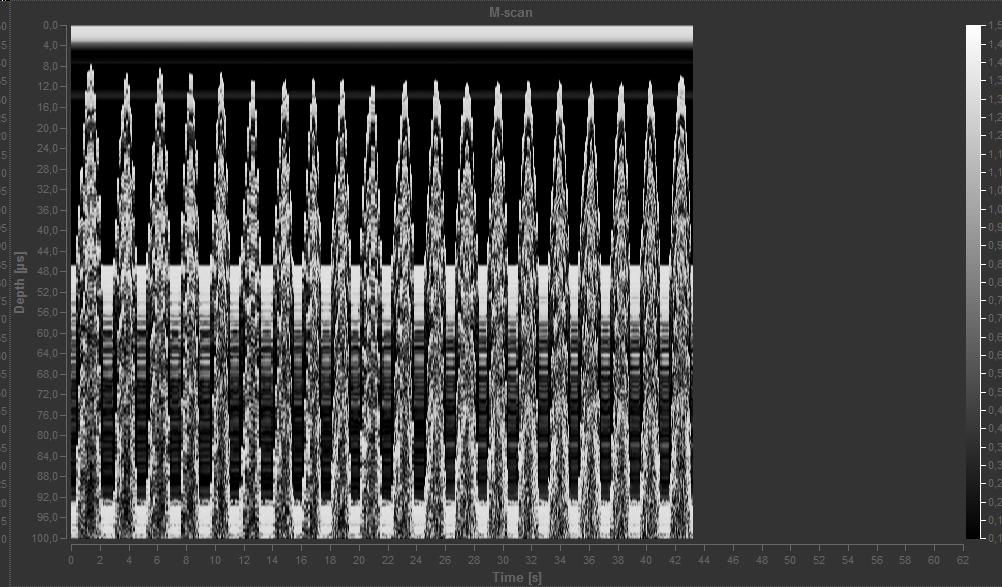
\includegraphics[height=7cm]{TM-Scan.PNG}
  \caption{Abbildung des TM-Scans für den simulierten Herzschlag.}
  \label{fig:TM}
\end{figure}

\begin{table}[H]
  \centering
  \caption{Gemessene Amplituden bei Herzschlagsimulation.}
  \label{tab:1}
  \begin{tabular}{c c c }
    \toprule
  Schlag & $t_s/\symup{\mu s}$ & $V_s/\symup{cm^3}$ \\
    \midrule
    1  &  38,96 & 40,17     \\
    2  &  37,22 & 37,32     \\
    3  &  38,58 & 39,54     \\
    4  &  37,60 & 37,93     \\
    5  &  37,80 & 38,26     \\
    6  &  36,44 & 36.09     \\
    7  &  36,45 & 36,11     \\
    8  &  36,47 & 36,14     \\
    9  &  36,46 & 36,12     \\
    10 &  35,26 & 34,28      \\
    11 &  36,24 & 35,78     \\
    12  &  36,24 & 35,78     \\
    13  &  35,86 & 35,19     \\
    14  &  35,90 & 35,26     \\
    15  &  36,04 & 35,47     \\
    16  &  36,04 & 35,47     \\
    17  &  36,01 & 35,42     \\
    18  &  36,01 & 35,42     \\
    19  &  36,24 & 35,78     \\
    20  &  37,42 & 37,64     \\
    \bottomrule
  \end{tabular}
\end{table}

Als Mittelwert ergibt sich ein Volumen von $V_{m} = (36,46 \pm 1,49) \: \symup{cm^3}$.

Aus
\begin{equation*}
  V_{Herz} = V_m \cdot f
\end{equation*}
ergibt sich das gesuchte Herzvolumen zu
\begin{equation*}
  V_{Herz} = (17,1 \pm 0,7) \: \symup{\frac{cm^3}{s}}
\end{equation*}
